\section{Problembeskrivelse}
\label{sec:issue}

En operasjonsforsterker (opamp) er en krets med fem tilkobligspunkter som vist i figur \ref{fig:01opamp} a)  og med en modell som vist i figur \ref{fig:01opamp} b).

\begin{figure}[!hbt]
	\centering
	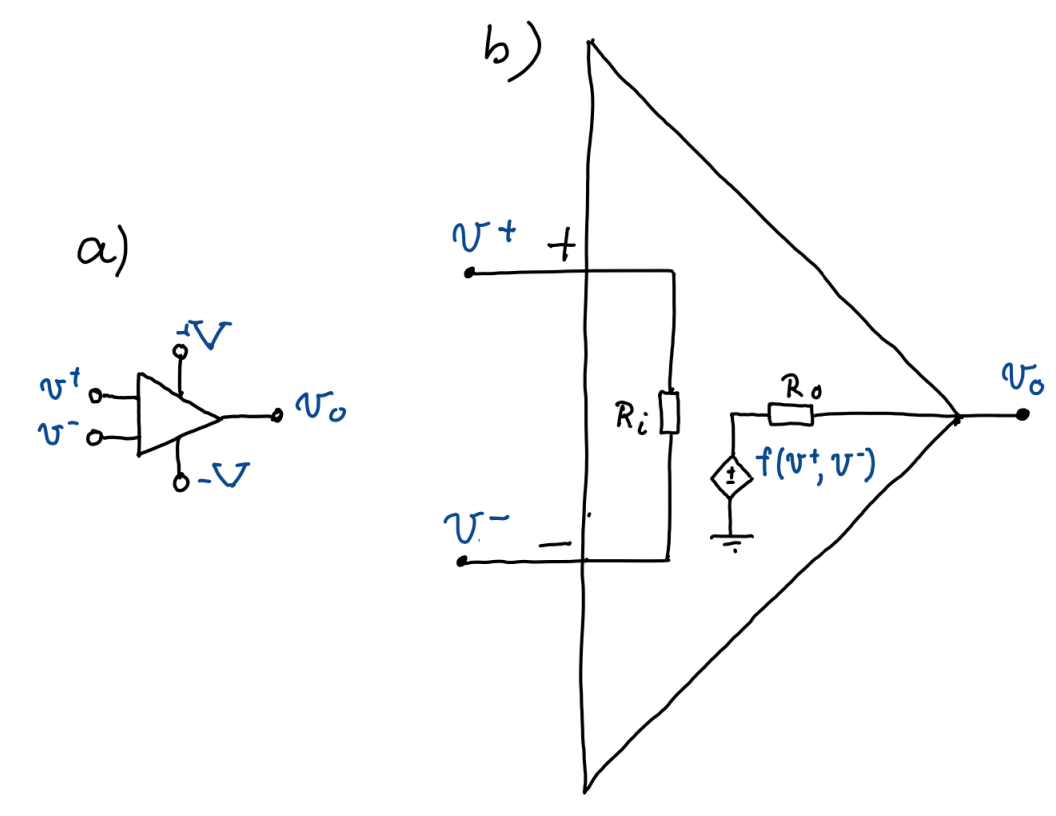
\includegraphics[scale=0.5]{./Images/01Issue/01_opamp.png}
	\caption{Operasjonsforsterker: a) symbol, b) modell.}
	\label{fig:01opamp}
\end{figure}

en \textit{ideell} opamp har følgende egenskaper:
\begin{enumerate}
    \item inngangsmotstanden $R_i$ er uendelig stor
    \item utgangsmotstanden $R_o = 0$
    \item utgangen er gitt som \newline \begin{equation} v_o=f(v^+,v^-) = \biggl\{ {{min\{V,A(v^+-v^-)\}} \atop {max\{V,A(v^+-v^-)\}}} {{\text{for } v^+-v^->0}\atop{\text{for } v^+-v^-<0}} \label{eq:v_o} \end{equation} \newline dvs. som vist i figur \ref{fig:02karakteristikk} Konstanten A er opampens \textit{åpen løkke-forsterking}. En reell operasjonsforsterker er et elektronisksystem som i større eller mindre grad oppfyller betingelesene ovenfor. Typiske avvik er at inngangs- og utgangsmotstandene har endelige verdier. Videre er utgangen gitt som en funksjon. \newline \begin{equation} v_o=f(v^+,v^-) \end{equation} \newline som ikke eksakt oppfyller den vi har i \ref{eq:v_o}.
\end{enumerate}

\begin{figure}[!hbt]
	\centering
	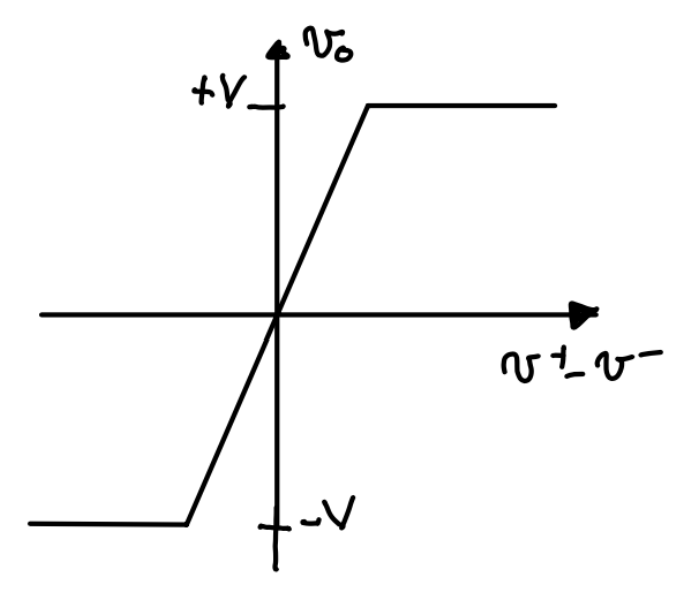
\includegraphics[scale=0.5]{./Images/01Issue/02_karakteristikk.png}
	\caption{ Karakteristikk for ideell operasjonsforsterker.}
	\label{fig:02karakteristikk}
\end{figure}

Operasjonsforsterkeren som designes i dette forsøket skal vurderes utifra:

\begin{enumerate}
	\item Inngangsmotstand
	\item Utgangsmotstand
	\item Forsterking A ved sinuspåtrykk med frekvens $f = 1 kHz$
	\item Total harmonisk distorsjon ved sinuspåtrykk med frekvens $f = 1 kHz$
\end{enumerate}

De to siste punktene skal undersøkes ved to forskjellige lastmotstander: $R_L$ = 100 kohm og $R_L$ = 100 ohm. 
\newline Forsyninsspenning skal være ±5 volt. 
\newline Det skal også undersøkes hvor godt kretsløsningen virker som opamp i en ikke-inverterende forsterkerkobling med forsterking 10. Denne forsterkerkoblingen skal også undersøkes med hensyn på inngangs- og utgangsmotstand, samt total harmonisk distorsjon. Som for åpen løkkeforsterking, skal oppførselen undersøkes med de samme to lastmotstandene $R_L$ = 100 kohm og $R_L$ = 100 ohm.